\documentclass{article}
\usepackage[utf8]{inputenc}
\usepackage{datetime}
\usepackage{enumerate}
\usepackage{textcomp}
\usepackage{amsmath}
\usepackage{tikz}
\usetikzlibrary{arrows}
\usepackage{graphicx}
\usepackage{amssymb}
\graphicspath{ {./images/} }
   
\title{\bf \Large ASSIGNMENT 6}
\author{Xinhao Luo}
\date{\today}

\def\math#1{$#1$} 

\setlength{\textheight}{8.5in}
\setlength{\textwidth}{6.5in}
\setlength{\oddsidemargin}{0in}
\setlength{\evensidemargin}{0in}
\voffset0.0in

\begin{document}
\maketitle
\medskip

\section{Exercise 3.4}
\begin{enumerate}[a)]
    \item From (3.6), we have \math{\hat{y} = Hy} where \math{H = X(X^TX)^{-1}X^T}. We also have \math{Y = Xw^* + \epsilon}
        \begin{equation}
            \begin{split}
                \hat{y} &= X(X^TX)^{-1}X^T(Xw^* + \epsilon) \\
                &= X(X^TX)^{-1}X^TXw^* + X(X^TX)^{-1}X^T\epsilon \\
                &= Xw^* + H\epsilon
            \end{split}
        \end{equation}
    \item \begin{equation}
        \begin{split}
            \hat{y} - y &= (Xw^* + H\epsilon) - (Xw^* + \epsilon) \\
            &= H\epsilon - \epsilon \\
            &= (H - I) \epsilon
        \end{split}
    \end{equation}
    The matrix \math{H - I}, where \math{I} is identity matrix.
    \item Based on (3.3),
        \begin{equation}
            \begin{split}
                E_{in}(w_{lin}) &= \frac{1}{N} \|\hat{y} - y\|^2 \\
                &= \frac{1}{N} \|(H - I) \epsilon\|^2 \\
                &= \frac{1}{N} \epsilon^T(H - I)^T(H - I)\epsilon
            \end{split}
        \end{equation}
        From 3.3(c), we know that the \math{(I - H)^K = I - H}. As \math{H - I} is symmetric, \math{(H - I)^T = (H - I)}, so we may have \math{(H - I)^T(H - I) = (H - I)^2 = (I - H)^2 = (I - H)}
        \begin{equation}
            \begin{split}
                E_{in}(w_{lin}) &= \frac{1}{N} \epsilon^T(H - I)^T(H - I)\epsilon \\
                &= \frac{1}{N} \epsilon^T(I - H)\epsilon
            \end{split}
        \end{equation}
    \item  
        \begin{equation}
            \begin{split}
                E_D[E_{in}(w_{lin})] &= E_D[\frac{1}{N} \epsilon^T(I - H)\epsilon]\\
                &= \frac{1}{N} (E_D[\epsilon^T\epsilon] - E_D[\epsilon^TH\epsilon])
            \end{split}
        \end{equation}
        \math{E_D[\epsilon^T\epsilon] = N * \sigma^2} since \math{\epsilon} has zero means and \math{\sigma^2} variance. \math{E_D[\epsilon^TH\epsilon] = trace(H)\sigma^2} where \math{trace(H) = d + 1} from 3.3(d). Thus, % why E_D[\epsilon^TH\epsilon] -> trace(H) ?
        \begin{equation}
            \begin{split}
                E_D[E_{in}(w_{lin})] &= \frac{1}{N} (E_D[\epsilon^T\epsilon] - E_D[\epsilon^TH\epsilon]) \\
                &=\frac{1}{N} (\sigma^2 - (d + 1)\sigma^2) \\
                &= \sigma^2 (1 - \frac{d + 1}{N})
            \end{split}
        \end{equation}
    \item 
        \begin{equation}
            \begin{split}
                E_{D, \epsilon'}[E_{test}(w_{lin)}] &= E_{D, \epsilon'}[\frac{1}{N}\|Xw - y'\|^2] \\
                &= \frac{1}{N} E_{D, \epsilon'}[\|Xw^* + H\epsilon - (Xw^* + \epsilon')\|^2] \\
                &= \frac{1}{N} E_{D, \epsilon'}[\|H\epsilon - \epsilon'\|^2] \\
                &= \frac{1}{N} E_{D, \epsilon'}[\|\epsilon^TH^TH\epsilon - 2\epsilon^TH^T\epsilon' + \epsilon'^T\epsilon'\|] \\ 
                &= \frac{1}{N} (\sigma^2(d + 1) + N\sigma^2) \\
                &= \sigma^2(1 + \frac{d+1}{N})
            \end{split}
        \end{equation}
    Here, we know that \math{\epsilon} and \math{\epsilon'} share the same mean and variance, so \math{\epsilon'^T\epsilon = N\sigma^2} from (d).\\ As \math{H} is symmetry, we may also have \math{\epsilon^TH^TH\epsilon = \epsilon^TH\epsilon}, where from (d) we know it is \math{(d + 1)\sigma^2}. \\
    As \math{\epsilon} and \math{\epsilon'} are independent and have zero means, \math{\epsilon^TH^T\epsilon'} is expected to be zero.
\end{enumerate}

\section{Problem 3.1}

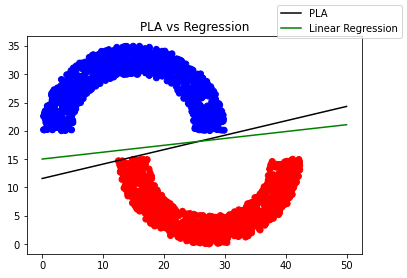
\includegraphics[]{3.1/1}

\begin{enumerate}
    \item For PLA, we have \math{y = -0.2544473141298261x + 11.586525302316833}
    \item For Linear Regression, we have \math{-1.15950148 + -0.00936171x + 0.0771953y = 0}
\end{enumerate}

Both methods have successfully found the solutions though different ones. The PLA stop at the first iteration separates the data while linear regression find the one with the shortest distance.

\section{Problem 3.2}

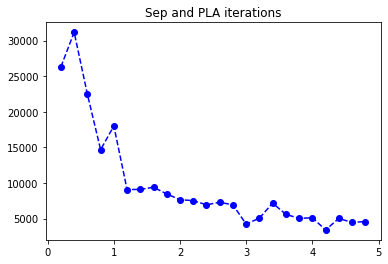
\includegraphics[]{3.2/1}

The number of iterations is decreasing while the sep is increasing, which match the inverse relation from problem (1.3).

\section{Problem 3.8}

\begin{equation}
    \begin{split}
        E_{out}(h) &= E[(h(x) - y)^2] \\
        &= E[((h(x) + h^*(x)) - (h^*(x) - y))^2] \\
        &= E[(h(x) - h^*(x))^2] + 2E[(h(x) - h^*(x))(h^*(x) - y)] + E[(h^* - y)^2] \\
        &= E[(h(x) - h^*(x))^2] + E[(h^*(x) - y)^2] \\
        &\leq E[(h^*(x) - y)^2]
    \end{split}
\end{equation}

From \math{E[E[y|x]] = E[y]}, \math{E[(h(x) - h^*(x))(h^*(x) - y)] = E[(h(x) - h^*(x))]E[(h^*(x) - y)|x]}. Then \math{E[h^*(x) - y|x] = E[h^*(x)|x] - E[y|x] = 0}. \\

Thus, we may have

\begin{equation}
    \begin{split}
        E[\epsilon(x)] &= E[E[\epsilon(x)|x]] \\
        &= E[E[\hat{y} - y|x]] \\
        &= E[h^*(x) - h^*(x)] \\
        &= E[0] \\
        &= 0
    \end{split}
\end{equation}

\section{Handwritten data}

\begin{enumerate}[a)]
    \item 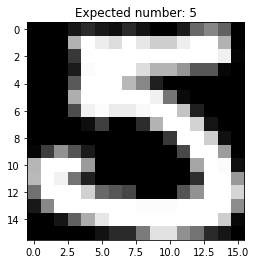
\includegraphics[]{images/hand/1} 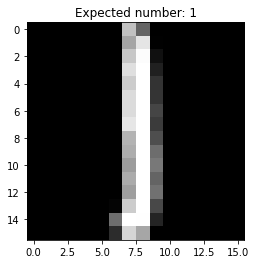
\includegraphics[]{images/hand/2}
    \item Here I choose the up-down symmetry and intensity here. Definitions are: 
        \begin{itemize}
            \item [symmetry] \math{\sum_{i = 0}^{15}\sum_{j = 0}^{15}|pixel[i][j] - pixel[15 - i][j]|} 
            \item [intensity] \math{\sum_{i = 0}^{15}\sum_{j = 0}^{15}pixel[i][j]}
        \end{itemize}
    \item 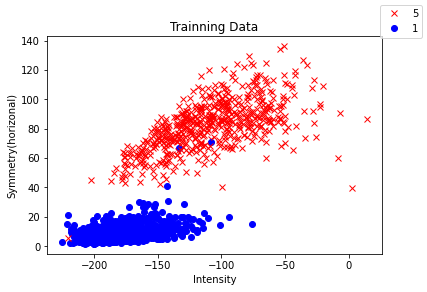
\includegraphics[]{images/hand/3} \\ 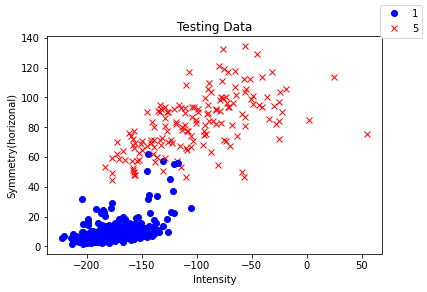
\includegraphics[]{images/hand/4}
\end{enumerate}

\end{document}
